\documentclass[10pt,a4paper]{article}
\usepackage[T1]{fontenc}
\usepackage[utf8]{inputenc}
\usepackage{lmodern}
\usepackage{microtype}
\usepackage[margin=0.72in]{geometry}
\usepackage{graphicx}
\usepackage{booktabs}
\usepackage{array}
\usepackage{amsmath}
\usepackage[hidelinks]{hyperref}
\usepackage{titlesec}
\usepackage{caption}
\usepackage{enumitem}
\usepackage{textcomp}
\usepackage{hyperref}

\titleformat{\section}{\normalfont\large\bfseries}{\thesection}{0.55em}{}
\titlespacing*{\section}{0pt}{0.9em}{0.35em}
\titleformat{\subsection}{\normalfont\normalsize\bfseries}{\thesubsection}{0.5em}{}
\titlespacing*{\subsection}{0pt}{0.65em}{0.25em}
\captionsetup{font=small,labelfont=normalfont,textfont=normalfont,skip=3pt}
\setlist[itemize]{leftmargin=1.3em,itemsep=1pt,topsep=2pt,parsep=0pt}
\setlist[enumerate]{leftmargin=1.5em,itemsep=1pt,topsep=2pt,parsep=0pt}
\setlength{\textfloatsep}{7pt plus 2pt minus 2pt}
\setlength{\intextsep}{7pt plus 2pt minus 2pt}
\setlength{\floatsep}{6pt plus 2pt minus 2pt}
\setlength{\abovecaptionskip}{3pt}
\setlength{\parindent}{1.2em}
\setlength{\parskip}{0pt}
\pagestyle{plain}
\raggedbottom

\begin{document}

\begin{center}
{\LARGE\bfseries Technical Report of MK-UNet}\\[3pt]
{\large Evaluation on ClinicDB and ColonDB}\\[4pt]
{\small Step 1 - Deliverable 2}\\[3pt]
{\normalsize M. Mohaiminul Islam}\\[3pt]
{\footnotesize Paper: Rahman \& Marculescu, MK-UNet (ICCV) \quad--\quad
Code: \href{https://github.com/SLDGroup/MK-UNet.git}{SLDGroup/MK-UNet}}
\end{center}
\vspace{0.25em}

\section{Objective and Paper Overview}

This study reproduces part of the MK-UNet experiments and checks the released code against the paper. The public repository provides the polyp pipeline, so the experiments were run on ClinicDB and ColonDB using MK-UNet-T. The main goal was not only to get a DICE score, but also to understand the training process, check the model structure, and find reproducibility issues.

MK-UNet is a five-stage U-shaped CNN for lightweight medical image segmentation [1]. The standard model is reported with 0.316 M parameters and 0.314 G FLOPs. The paper reports an average DICE of 89.75\% across six datasets. The tiny model, MK-UNet-T, is reported with 0.027 M parameters and 0.062 G FLOPs. The main parts of the model are:

\begin{itemize}
\item MKDC: parallel depth-wise convolutions with different kernel sizes, followed by summation and channel shuffle.
\item MKIR: an inverted residual block that uses MKDC to extract features with different kernel sizes.
\item MKIRA: channel attention, spatial attention, and MKIR in the decoder to improve the features.
\item GAG: a grouped attention gate that filters skip-connection features before they are combined with the decoder features.
\end{itemize}

The multi-kernel design is an important part of the method. In the paper's BUSI ablation, the DICE score increases from 70.83 with a single $1\times1$ kernel to 78.04 with the kernel set $\{1,3,5\}$ [1].

\section{Reproduction Protocol}

\subsection{Code and environment}

Training was done on Windows 11 using an Intel i9-14900 CPU, 32 GB RAM, Python 3.8.20, and PyTorch 1.11.0+cu113. No GPU was used. The released code had fixed CUDA calls, so six \texttt{.cuda()} calls were changed to \texttt{.to(device)}. Checkpoint loading was also given \texttt{map\_location}, and a device option was added. Options for seed, number of runs, dataset, data path, augmentation, and resume were also added for controlled experiments. These changes were made to support reproducible CPU runs. The model architecture, loss, and metric formulas were not changed.

The ClinicDB split was 489/61/62 and the ColonDB split was 303/38/38 for train/validation/test. These splits match the 80:10:10 split described in the paper.

\subsection{Paper and repository settings}

The paper and the released training code use different training settings. Table~1 shows the main differences. For the benchmark runs in this study, the default training settings from the repository were used, but only one fixed run was done with seed 42.

\begin{table}[h]
\centering\small
\caption{Main differences between the paper and the released training script.}
\begin{tabular}{@{}lll@{}}
\toprule
Setting & Paper [1] & Run used here \\
\midrule
Learning rate & $1\times10^{-4}$ & $5\times10^{-4}$ + cosine scheduler \\
Batch size & 16 & 8 \\
Augmentation & none stated & rotation and flips enabled \\
Number of runs & five-run mean & one run, seed 42 \\
Epochs & 200 & 200 \\
Optimizer & AdamW & AdamW \\
\bottomrule
\end{tabular}
\end{table}

Parameter counts were checked before training. The measured values for the five variants were 0.0274 M, 0.0930 M, 0.3156 M, 1.1502 M, and 3.7581 M. These values match the paper's reported values to the shown precision. This gives a useful check that the model structure is correct. Measured FLOPs were about 5--8\% higher than the paper's values across the variants. This difference may be caused by the FLOP-counting method, but the exact reason was not determined in this study.

\newpage
\section{Experimental Results}

\begin{figure}[h]
\centering
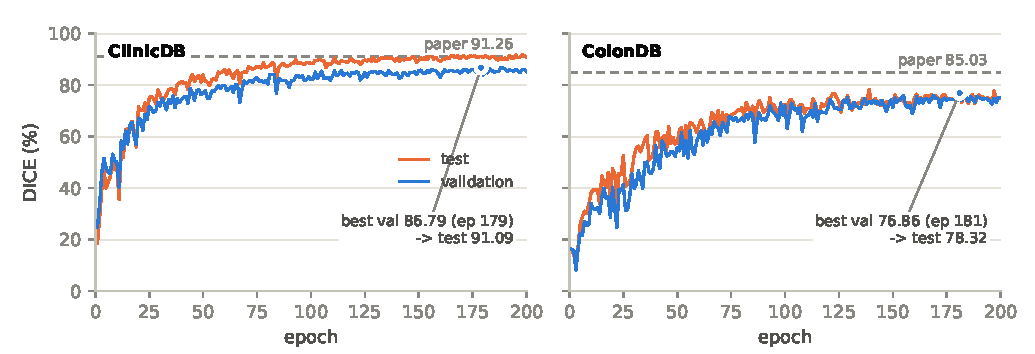
\includegraphics[width=0.97\linewidth]{figures/curves.pdf}
\caption{Training curves for 200 epochs using one run with seed 42. The checkpoint was selected using validation DICE. The released script also evaluates the test split at every epoch; test values were not used for checkpoint selection or tuning.}
\end{figure}

Both datasets used the same run settings. ClinicDB reached a test DICE of 91.09 and IoU of 84.63. ColonDB reached a test DICE of 78.32 and IoU of 69.46. The best validation DICE values were 86.79 at epoch 179 for ClinicDB and 76.86 at epoch 181 for ColonDB.

\begin{table}[h]
\centering\small
\caption{Published MK-UNet-T results and the single-run results obtained in this study.}
\begin{tabular}{@{}lrrrr@{}}
\toprule
Dataset & Paper DICE & Our DICE & Our IoU & Difference \\
\midrule
ClinicDB & 91.26 & 91.09 & 84.63 & -0.17 \\
ColonDB & 85.03 & 78.32 & 69.46 & -6.71 \\
\bottomrule
\end{tabular}
\end{table}

\begin{figure}[h]
\centering
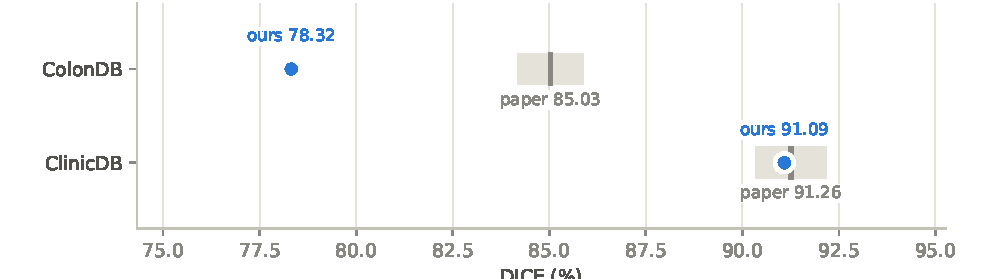
\includegraphics[width=0.72\linewidth]{figures/vs_paper.pdf}
\caption{Published five-run means and the single-run values obtained here. The shaded range is an illustrative reference based on the upper end of the paper's reported 1--4\% run-to-run variation. It is not a confidence interval and not a dataset-specific standard deviation.}
\end{figure}

The ClinicDB result is 0.17 DICE points below the published mean. Because this study used one seed and a different training protocol from the paper, this result should be described as numerically consistent with the published result, not as an exact reproduction.

The ColonDB result is 6.71 DICE points below the published mean. The paper reports 1--4\% standard deviations across its five-run results, but it does not provide a separate standard deviation for ColonDB. Therefore, this study cannot establish statistical significance from the published information alone. The ColonDB training curve reaches a stable plateau, which makes a major optimization failure less likely. However, this does not rule out effects from the training protocol, preprocessing, augmentation, or random seed.

Three possible explanations were not tested: the smaller ColonDB training set may be more sensitive to the differences in the training protocol; the repository-default augmentation may affect the tiny model differently on ColonDB; and ColonDB may have larger differences between random seeds. The most useful next experiment is to run ColonDB with the paper's exact settings using several seeds.

\section{Codebase and Reproducibility Findings}
\subsection{Per-image variation}

\begin{figure}[h]
\centering
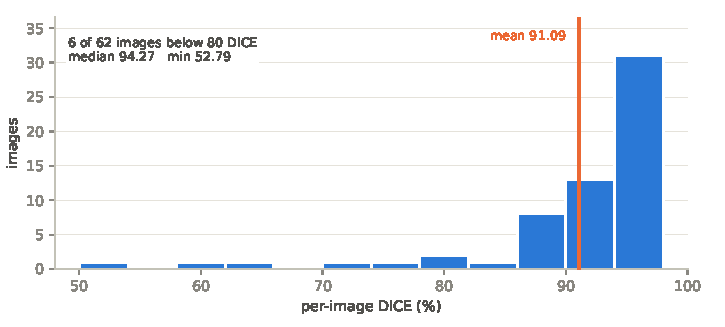
\includegraphics[width=0.61\linewidth]{figures/dist_clinicdb.pdf}
\caption{Per-image DICE on the ClinicDB test set. The mean is 91.09, the median is 94.27, six of 62 images are below 80, and the minimum is 52.79.}
\end{figure}

The ClinicDB mean does not show the full error pattern. Most test images have high scores, but a small number of images have low scores. This shows that per-image analysis is useful in addition to the mean DICE score.

\subsection{Unused auxiliary prediction heads}

The forward pass computes four segmentation outputs, but only the final output is returned for binary segmentation. A gradient check showed that 31 parameters in \texttt{out1/out2/out3} received no gradient in this setting. These heads therefore add extra computation during the binary runs used here. The paper recommends deep supervision for multi-class segmentation, so these heads may still be useful in a different training setting.

\subsection{Narrow channel-attention bottleneck in MK-UNet-T}

The released code uses channel-attention reduction ratios of 16, 16, 16, 8, and 4 across the five decoder stages. With MK-UNet-T channels $[4,8,16,24,32]$, the hidden attention width becomes 1 in four of the five stages. This creates a very narrow attention bottleneck in the tiny model. The standard model does not become this narrow. The paper describes a single reduction ratio of 16, while the code uses different ratios for different stages. Raising the minimum hidden width to 4 would add 440 parameters, about 1.6\% of MK-UNet-T's parameter count.

The code also uses one spatial-attention module across all decoder stages, while the channel-attention modules are different for each stage. This is another implementation detail that is not clearly described in the paper.

\section{Limitations and Link to the Path A Extension}

This reproduction has four main limitations. Only one seed was used for each dataset, while the paper reports five-run means. The default training settings from the repository were used instead of the exact settings from the paper. Training was done only on a CPU, so the runtime cannot be compared with the paper's GPU results. The checked version of the repository also provides only the polyp pipeline used here, so the other four benchmarks could not be reproduced in this setup.

The code audit found one direct methodological question in MKDC. The original block always computes the $1\times1$, $3\times3$, and $5\times5$ branches and uses the same sum for every input. The Step 2 Path A proposal develops this idea into MK-UNet-CC. It first tests input-dependent branch weights as a control. It then tests predictive entropy as an additional routing signal, annealed top-1 routing that skips unused branches during inference, and routing-guided pruning for a smaller static model. Adaptive weighting itself is not treated as the main novelty. The main question is whether conditional branch execution is useful for the very small MK-UNet-T model and whether lower FLOPs also lead to lower real latency. The Step 2 preliminary results are reported separately and do not change the interpretation of this Step 1 reproduction.

\section*{References}
\footnotesize

[1] M. M. Rahman and R. Marculescu, ``MK-UNet: Multi-kernel Lightweight CNN for Medical Image Segmentation,'' arXiv:2509.18493, 2025.

[2] SLDGroup, ``MK-UNet,'' public code repository. \url{https://github.com/SLDGroup/MK-UNet.git}

\end{document}
